\begin{figure}[h] 
\centering 
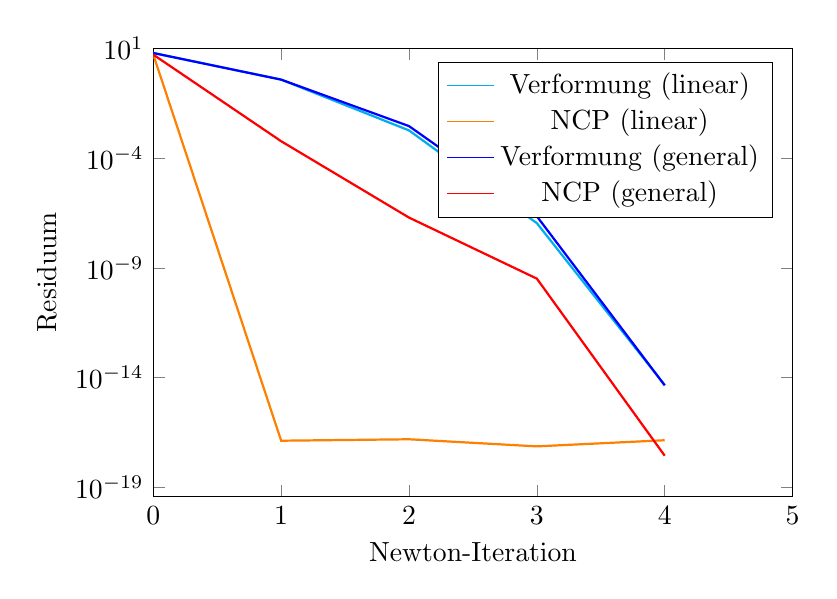
\begin{tikzpicture}[every plot/.append style={thick}] 
\begin{axis}[ 
label style={font=\normalsize}, 
xlabel={Newton-Iteration}, 
ylabel={Residuum}, 
xmin=0, xmax=5, 
ymode=log, 
ymin=0, ymax=10, 
width=0.8\textwidth, 
height=0.6\textwidth, 
legend pos=north east, 
legend style={cells={align=left}}, 
grid style=dashed, 
] 
\addplot[ 
color=cyan, 
] 
coordinates { 
(0, 6.02e+00)(1, 3.71e-01)(2, 1.80e-03)(3, 1.08e-07)(4, 4.61e-15)}; 
\addlegendentry{Verformung (linear)} 
\addplot[ 
color=orange, 
] 
coordinates { 
(0, 5.06e+00)(1, 1.35e-17)(2, 1.57e-17)(3, 7.46e-18)(4, 1.42e-17)}; 
\addlegendentry{NCP (linear)} 
\addplot[ 
color=blue, 
] 
coordinates { 
(0, 6.01e+00)(1, 3.69e-01)(2, 2.83e-03)(3, 2.22e-07)(4, 4.47e-15)}; 
\addlegendentry{Verformung (general)} 
\addplot[ 
color=red, 
] 
coordinates { 
(0, 5.06e+00)(1, 5.80e-04)(2, 1.94e-07)(3, 3.22e-10)(4, 2.80e-18)}; 
\addlegendentry{NCP (general)} 
\end{axis} 
\end{tikzpicture} 
\caption{Residuen des Stoffgesetzes 'Neo Hooke' mit Hinderniss 'Parabel' und 50 Freiheitsgraden für die Verschiebung.} 
\label{fiq:NeoHooke_Parabel_level1} 
\end{figure} 
